\documentclass[a4paper, 10pt]{article}

\title{MOSIG M1 Visual Computing TP4}
\date{}
\author{Gilchrist N'dri \and Quoc-Trung Vuong}

\usepackage[utf8]{inputenc}
\usepackage{listings}
\usepackage{color}
\usepackage{amsmath}
\usepackage{graphicx}
\usepackage{geometry}

\geometry{a4paper, portrait, margin=1in}

\definecolor{dkgreen}{rgb}{0,0.6,0}
\definecolor{gray}{rgb}{0.5,0.5,0.5}
\definecolor{mauve}{rgb}{0.58,0,0.82}

\lstset{
  language=C,
  showstringspaces=false,
  columns=flexible,
  basicstyle={\small\ttfamily},
  numbers=none,
  numberstyle=\tiny\color{gray},
  keywordstyle=\color{blue},
  commentstyle=\color{dkgreen},
  stringstyle=\color{mauve},
  otherkeywords={},
  breaklines=true,
  breakatwhitespace=true,
  tabsize=2
}

\begin{document}
\maketitle

\paragraph{Test subject} All illustrations used in this report are results of the respective operation applied on the boat image \texttt{boat\_noise.pgm} from TP2. The image is filtered using binomial filter with size of $3\times3$ for 5 times.
\begin{figure}[!htb]
\centering
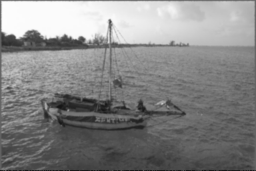
\includegraphics[width=256px]{boat3x3_5.png}
\caption{Test subject}
\label{fig-subject}
\end{figure}


\section{Gradient}
\subsection{Approximate gradient using Sobel operator}
\paragraph{} We apply Sobel operator ($3\times3$) on the image to obtain its approximate gradient of each pixel along each axis: horizontal ($x$) and vertical ($y$)
\subsubsection{$x$-axis}
\paragraph{} The approximate gradient on each pixel $(m,n)$ is computed by the following formula:
\begin{equation}
I_x(m,n) = \sum_{i=m-1}^{m+1}\sum_{j=n-1}^{n+1}{h_x(i-(m-1),j-(n-1)) * I(i,j)}
\end{equation}
with coefficient $h_x$ being:
\begin{equation}
h_x = \frac{1}{4} * \left[
\begin{matrix}
-1 & 0 & 1 \\
-2 & 0 & 2 \\
-1 & 0 & 1
\end{matrix}
\right]
\end{equation}

For pixels on each border, we set the gradient to be $0$.

\paragraph{Implementation}
We use the same function for computing gradient on both direction for each pixel, with the last argument specifying the mask to apply filter on.
\begin{lstlisting}[frame=single]
float gradient_1d(gray *map, int i, int j, int rows, int cols, float *mask) {
  if (i - 1 < 0 || i + 1 >= rows || j - 1 < 0 || j + 1 >= cols) {
    return 0;
  }

  float val = 0.0f;
  for (int i1 = i - 1; i1 <= i + 1; i1++) {
    for (int i2 = j - 1; i2 <= j + 1; i2++) {
      int mask_index = (i1 - i + 1) * 3 + (i2 - j + 1);
      int img_index = i1 * cols + i2;
      val += (float) map[img_index] * mask[mask_index];
    }
  }
  return val;
}
\end{lstlisting}

The function to obtain Sobel filter mask for $x$-axis:
\begin{lstlisting}[frame=single]
float *sobel_mask_x() {
  float *mask = malloc(sizeof(float) * 9);
  mask[0] = -1.0f / 4;
  mask[1] = 0;
  mask[2] = 1.0f / 4;
  mask[3] = -2.0f / 4;
  mask[4] = 0;
  mask[5] = 2.0f / 4;
  mask[6] = -1.0f / 4;
  mask[7] = 0;
  mask[8] = 1.0f / 4;
  return mask;
}
\end{lstlisting}

Put them together to compute the whole image gradient:
\begin{lstlisting}[frame=single]
float *grad_x_image = malloc(cols * rows * sizeof(float));
for (i = 0; i < rows; i++) {
  for (j = 0; j < cols; j++) {
    grad_x_image[i * cols + j] = gradient_1d(graymap, i, j, rows, cols, sobel_mask_x());
  }
}
\end{lstlisting}

\subsubsection{$y$-axis}
\paragraph{} The approximate gradient on each pixel $(m,n)$ is computed by the following formula:
\begin{equation}
I_y(m,n) = \sum_{i=m-1}^{m+1}\sum_{j=n-1}^{n+1}{h_y(i-(m-1),j-(n-1)) * I(i,j)}
\end{equation}
with coefficient $h_y$ being:
\begin{equation}
h_y = \frac{1}{4} * \left[
\begin{matrix}
-1 & -2 & -1 \\
0 & 0 & 0 \\
1 & 2 & 1
\end{matrix}
\right]
\end{equation}

The gradient on border pixels is set to $0$.

\paragraph{Implementation}
We apply the same method as with Sobel filter on $x$-axis. The filter mask is replaced with:
\begin{lstlisting}[frame=single]
float *sobel_mask_y() {
  float *mask = malloc(sizeof(float) * 9);
  mask[0] = -1.0f / 4;
  mask[1] = -2.0f / 4;
  mask[2] = -1.0f / 4;
  mask[3] = 0;
  mask[4] = 0;
  mask[5] = 0;
  mask[6] = 1.0f / 4;
  mask[7] = 2.0f / 4;
  mask[8] = 1.0f / 4;
  return mask;
}
\end{lstlisting}

\subsection{Gradient images}
\paragraph{} The gradient values $I_x$ and $I_y$ can be either positive or negative, and we are not sure how large its absolute value can be. Therefore, we need to apply stretching (or shrinking) to translate their value range to $(0, 255)$ for display purpose.

The function below takes an array of real numbers and translate them to $(0, maxval)$ scale:
\begin{lstlisting}[frame=single]
gray *float_to_image(float *gradient, int rows, int cols) {
  float min_mag = 0;
  float max_mag = 0;
  for (int i=0; i<rows * cols; i++) {
    if (gradient[i] > max_mag) {
      max_mag = gradient[i];
    }
    if (gradient[i] < min_mag) {
      min_mag = gradient[i];
    }
  }

  gray *out = malloc(rows * cols * sizeof(gray));
  for (int i=0; i<rows; i++) {
    for(int j=0; j<cols; j++) {
      out[i * cols + j] = (gray) ((gradient[i * cols + j] - min_mag) / (max_mag - min_mag) * maxval);
    }
  }
  return out;
}
\end{lstlisting}

\paragraph{Results} The illustrations can be seen on Figure \ref{fig-gradient}.

\begin{figure}[!htb]
\centering
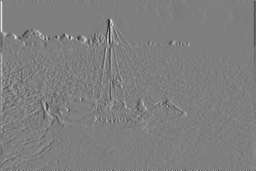
\includegraphics[width=192px]{boat3x3_5_grad_x.png}
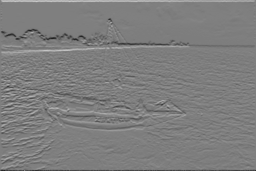
\includegraphics[width=192px]{boat3x3_5_grad_y.png}
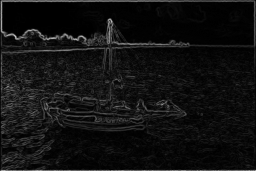
\includegraphics[width=192px]{boat3x3_5_grad_mag.png}
\caption{From left to right, gradient x, gradient y, gradient magnitude of the test subject}
\label{fig-gradient}
\end{figure}


\section{Interest Point Detection}
\subsection{Gradient $I^2_x$, $I^2_y$, $I_{xy}$}
We use the following functions computing $I^2_x$, $I^2_y$, and $I_{x,y}$ for each pixel $(i, j)$:

\begin{lstlisting}[frame=single]
float gradient_x2(gray *map, int i, int j, int rows, int cols) {
  float gradient_x = gradient_1d(map, i, j, rows, cols, sobel_x);
  return gradient_x * gradient_x;
}
\end{lstlisting}

\begin{lstlisting}[frame=single]
float gradient_y2(gray *map, int i, int j, int rows, int cols) {
  float gradient_y = gradient_1d(map, i, j, rows, cols, sobel_y);
  return gradient_y * gradient_y;
}
\end{lstlisting}

\begin{lstlisting}[frame=single]
float gradient_xy(gray *map, int i, int j, int rows, int cols) {
  float gradient_x = gradient_1d(map, i, j, rows, cols, sobel_x);
  float gradient_y = gradient_1d(map, i, j, rows, cols, sobel_y);
  return gradient_x * gradient_y;
}
\end{lstlisting}

\paragraph{Results} The illustrations can be seen on Figure \ref{fig-gradient-square}.

\begin{figure}[!htb]
\centering
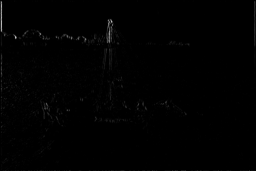
\includegraphics[width=192px]{boat3x3_5_grad_x2.png}
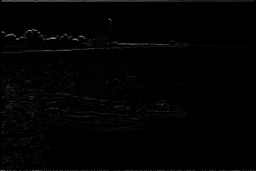
\includegraphics[width=192px]{boat3x3_5_grad_y2.png}
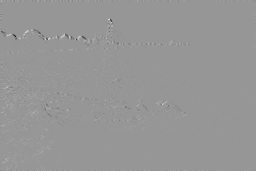
\includegraphics[width=192px]{boat3x3_5_grad_xy.png}
\caption{From left to right, gradient $I_x^2$, gradient $I_y^2$, gradient $I_{xy}$ of the test subject}
\label{fig-gradient-square}
\end{figure}

\subsection{Harris function}
The Harris function value for each pixel is computed by the following formula:
\begin{equation}
H = detC - \alpha * trace^2C
\label{eq-harris}
\end{equation}
with matrix $C$ being:
\begin{equation}
C = \left[
\begin{matrix}
I^2_x & I_{xy} \\
I_{xy} & I^2_y
\end{matrix}
\right]
\end{equation}

\paragraph{Implementation} We use the following function to compute the Harris value on each pixel:
\begin{lstlisting}[frame=single]
float *harris(float *grad_x2, float *grad_y2, float *grad_xy, float alpha, int rows, int cols) {
  float *out = malloc(rows * cols * sizeof(float));
  int index;
  float det;
  float trace;

  for (int i = 0; i < rows; i++) {
    for (int j = 0; j < cols; j++) {
      index = i * cols + j;
      det = grad_x2[index] * grad_y2[index] - grad_xy[index] * grad_xy[index];
      trace = grad_x2[index] + grad_y2[index];
      out[index] = det - alpha * trace * trace;
    }
  }

  return out;
}
\end{lstlisting}

This function is applied on a filtered version of $I^2_x$, $I^2_y$, $I_{xy}$ because without filtering, they always nullify each other when computing $detC$. Here we use binomial filter with $3\times3$-size neighborhood area.

\begin{lstlisting}[frame=single]
float *grad_x2_image_filtered = filter(grad_x2_image, rows, cols, binomial_3);
float *grad_y2_image_filtered = filter(grad_y2_image, rows, cols, binomial_3);
float *grad_xy_image_filtered = filter(grad_xy_image, rows, cols, binomial_3);

float *harris_image = harris(grad_x2_image_filtered, grad_y2_image_filtered, grad_xy_image_filtered, harris_alpha, rows, cols);
\end{lstlisting}


\paragraph{Results} The illustrations can be seen on Figure \ref{fig-harris}.

\begin{figure}[!htb]
\centering
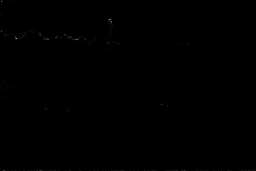
\includegraphics[width=192px]{boat3x3_5_harris_000.png}
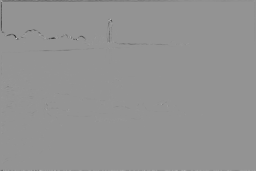
\includegraphics[width=192px]{boat3x3_5_harris_004.png}
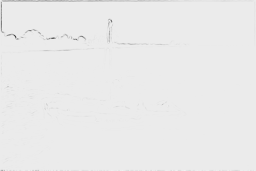
\includegraphics[width=192px]{boat3x3_5_harris_010.png}
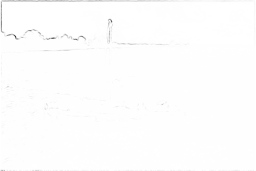
\includegraphics[width=192px]{boat3x3_5_harris_100.png}
\caption{From left to right, Harris function result with $\alpha=\{0, 0.04, 0.1, 1\}$ respectively}
\label{fig-harris}
\end{figure}

The illustrations are made of Harris values that are stretched to $(0, 255)$ range for display purposes. Before stretching, the majority of Harris values are $0$ on the \textit{non-interesting} parts of the original image. They are the \textit{background}, pixels with the most dominant intensity, of the output images. As can be seen from the output images, contours are displayed with lower intensity than the background, while corners are displayed with higher intensity. This means, the original Harris values for contours are negative while that for corners are positive. By changing the coefficient $\alpha$ in Harris formula (Equation \ref{eq-harris}), the contours can be blended into the background for low $\alpha$ (i.e $\alpha=0$), while the corners will become unrecognizable for high $\alpha$ (i.e $\alpha=1$).

\subsection{Maxima}
\subsubsection{Global Maxima}
To find global maxima, we sort the array of Harris values obtained from previous steps and retrieve the $n-th$ largest value. The output image is made by keeping pixel with Harris values higher than that $n-th$ largest value. Other pixels are set as 0.

We use the following function to compute global maxima:
\begin{lstlisting}[frame=single]
float *global_maxima(float *array, float *sorted_array, int nb_maxima, int rows, int cols) {
  int size = rows * cols;
  float *out = malloc(size * sizeof(float));
  for (int i = 0; i < size; i++) {
    if (array[i] < sorted_array[size - nb_maxima]) {
      out[i] = 0;
    } else {
      out[i] = array[i];
    }
  }
  return out;
}
\end{lstlisting}

and apply it on the output of Harris function from previous steps:
\begin{lstlisting}[frame=single]
float *harris_image = harris(grad_x2_image_filtered, grad_y2_image_filtered, grad_xy_image_filtered, harris_alpha, rows, cols);

// clone and sort (ascending order) the array of harris values
float *sorted_harris = malloc(cols * rows * sizeof(float));
memcpy(sorted_harris, harris_image, cols * rows * sizeof(float));
qsort(sorted_harris, cols * rows, sizeof(float), cmp_float);

float *harris_maxima = global_maxima(harris_image, sorted_harris, nb_maxima, rows, cols);
\end{lstlisting}

\paragraph{Result} The illustration can be seen on Figure \ref{fig-global}. We did scale down the original image to $192\times128$ before the procedure to make the maxima visible. Moreover, all maxima are set to highest intensity for better visibility as well.
\begin{figure}[!htb]
\centering
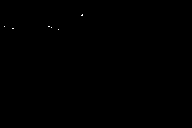
\includegraphics[width=192px]{boat3x3_5_global_10.png}
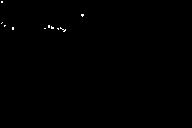
\includegraphics[width=192px]{boat3x3_5_global_50.png}
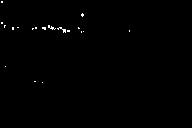
\includegraphics[width=192px]{boat3x3_5_global_100.png}
\caption{From left to right, 10/50/100 global maxima}
\label{fig-global}
\end{figure}

\subsubsection{Local Maxima}
To get local maxima, we perform the same operations as with global maxima, but require some preprocessing to only retain local maxima. We pass through every Harris value of each pixel, suppress the values are not local maxima (if the value at that pixel is not larger than all of its $3\times3$-neighbor area).

The function to suppress non local maxima:
\begin{lstlisting}[frame=single]
float *suppress_non_local_max(float *array, int rows, int cols) {
  float *out = malloc(rows * cols * sizeof(float));
  int index;
  for (int i = 0; i < rows; i++) {
    for (int j = 0; j < cols; j++) {
      index = i * cols + j;
      if (array[index] > array[(i - 1) * cols + j - 1]
        && array[index] > array[(i - 1) * cols + j]
        && array[index] > array[(i - 1) * cols + j + 1]
        && array[index] > array[i * cols + j - 1]
        && array[index] > array[i * cols + j + 1]
        && array[index] > array[(i + 1) * cols + j - 1]
        && array[index] > array[(i + 1) * cols + j]
        && array[index] > array[(i + 1) * cols + j + 1]
      ) {
        out[index] = array[index];
      } else {
        out[index] = 0;
      }
    }
  }
  return out;
}
\end{lstlisting}
and apply it:
\begin{lstlisting}[frame=single]
float *non_local_harris = suppress_non_local_max(harris_image, rows, cols);

// sort it (ascending order)
float *sorted_non_local_harris = malloc(cols * rows * sizeof(float));
memcpy(sorted_non_local_harris, non_local_harris, cols * rows * sizeof(float));
qsort(sorted_non_local_harris, cols * rows, sizeof(float), cmp_float);


float *harris_lmaxima = maxima(non_local_harris, sorted_non_local_harris, nb_maxima, rows, cols);
\end{lstlisting}

\paragraph{Result} The illustration can be seen on Figure \ref{fig-local}.
\begin{figure}[!htb]
\centering
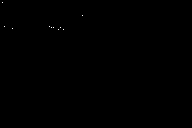
\includegraphics[width=192px]{boat3x3_5_local_10.png}
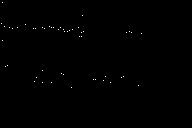
\includegraphics[width=192px]{boat3x3_5_local_50.png}
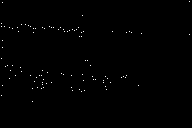
\includegraphics[width=192px]{boat3x3_5_local_100.png}
\caption{From left to right, 10/50/100 local maxima}
\label{fig-local}
\end{figure}

\end{document}